% LaTeX Article Template - using defaults
\documentclass[12pt]{article}
\usepackage{amsmath}
\usepackage{amssymb}
\usepackage{amsfonts}
\usepackage{amsthm}
\usepackage{mathrsfs}
\usepackage{graphicx}
\usepackage{subcaption}
\usepackage{pseudocode}

\pdfpagewidth 8.5in
\pdfpageheight 11in

\usepackage[final]{showkeys}


% Set left margin - The default is 1 inch, so the following 
% command sets a 1.25-inch left margin.
\setlength{\oddsidemargin}{0.25in}

% Set width of the text - What is left will be the right margin.
% In this case, right margin is 8.5in - 1.25in - 6in = 1.25in.
\setlength{\textwidth}{6in}

% Set top margin - The default is 1 inch, so the following 
% command sets a 0.75-inch top margin.
\setlength{\topmargin}{-0.25in}

% Set height of the text - What is left will be the bottom margin.
% In this case, bottom margin is 11in - 0.75in - 9.5in = 0.75in
\setlength{\textheight}{8in}

\theoremstyle{definition}
\newtheorem{definition}{Definition}[section]

% Set the beginning of a LaTeX document
\begin{document}

\title{Streaming Approximate Convex Hulls}         % Enter your title between curly braces
\author{Ananya Kumar}        % Enter your name between curly braces
\date{\today}          % Enter your date or \today between curly braces
\maketitle

\section{Problem}

Given a set of 2-dimensional points $P$, an $\epsilon$-approximate convex hull is a set $S$ such that every point in $P$ is within Euclidean distance $\epsilon$ from some point in $S$. Let OPT$(P, \epsilon)$ be the size of a smallest $\epsilon$-approximate convex hull of $P$. There is a very simple polynomial time algorithm that can find a smallest $\epsilon$-approximate convex hull. However, we are interested in streaming algorithms for this problem.
\\

\noindent Order the points in $P$ from $1$ to $n$. Let $P_{i:j}$ denote all points between indices $i$ and $j$, inclusive of $i$ and $j$. Let MAX-OPT$(P, \epsilon)$ be $\max_{1 \leq i \leq n} $OPT$(P_{1:i}, \epsilon)$. There has been a lot of past work on the streaming approximate convex hull problem, but we want a streaming algorithm that uses memory competitive with MAX-OPT. Note that we cannot get a streaming algorithm that is always competitive with OPT, because the optimal approximate convex hull for the first half of the points could be significantly larger than the optimal approximate convex hull for the whole set. 

\section{Goals}

This problem is very difficult, and we have come up with a bunch of ideas that do not seem to work in general. So we look at a few easier goals for now.

\begin{enumerate}
\item Can we solve the problem if the points come in random order? This is a reasonable assumption, because if the points were generated i.i.d. with respect to \emph{any generative process} then they would effectively come in random order.

\item Can we solve the problem if the points are generated or ordered in a specific way? For example, we have discussed some interesting generative models. What if $P$ contains the origin and points are ordered by angle to the $x$-axis?

\item Can we solve this problem in the case that $P$ has no interior points? An interior point $p \in P$ is inside the convex hull of $P \setminus \{p\}$.

\item Can we solve the problem when MAX-OPT is a small specified number? For example, the case where MAX-OPT is 2?

\end{enumerate}

In pursuit of these goals, we propose 2 algorithms and sketch out correctness arguments for them. We then discuss ideas for solving the more general cases. The main results are:

\begin{enumerate}

\item We give a simple algorithm that uses expected space $O($MAX-OPT$\cdot \log{n})$. We give intuition for a correctness argument.

\item We give a simple algorithm that, assuming there are no interior points, and the points come in clockwise (or anti-clockwise) order uses space $O($MAX-OPT$)$ space. We give a sketch of a correctness argument.

\end{enumerate}

\section{Random Order Algorithm}

\subsection{Pseudocode}

\begin{lstlisting}[escapechar=|]
S = {}
for p |$\in$| P:
  if dist(p, S) |$\leq$| |$\epsilon$|:
    // Discard p
  else:
    S = S |$\cup$| {p}
    Delete all interior points in P (see Goal 3)
\end{lstlisting}

\subsection{Proof Intuition}

\textbf{Correctness}: Let $S_i$ be $S$ after the $i^{\mbox{th}}$ iteration of the loop. Notice that the convex hull of $S_{i+1}$ always contains $S_i$. Essentially $S$ always gets strictly larger, because we only discard points in the convex hull of $S$. Then, a simple induction shows that $S$ always contains all points in $P$ within distance $\epsilon$.
\\

\noindent \textbf{1-D Space}: First, we note a lemma. Consider our algorithm running on a set of 1 dimensional points, except suppose that we don't delete interior points. The expected size of our set $S$ would be $\leq \log_2{n}$ (it follows from an inductive argument and the concavity of $\log$). 
\\

\noindent \textbf{2-D Space}: Consider an optimal $\epsilon$-approximate convex hull $O$. Let $A$ be the \"inner\" set of points that are contained inside $O$, but within distance $\epsilon$ of $O$. Let $B$ be the \"outer\" set of points that are outside of the convex polygon defined by $O$, but within distance $\epsilon$ of $O$. For example, in figure 1(a), $O$ defines a rectangle. The original set of points $P$ is not shown. $A$ is the region shaded in green in figure 1(b). In figure 1(b) we also marked the deep interior, the set of points contained in $O$ but not in $A$. $B$ is the region shaded in blue in figure 1(c). 
\\

\begin{figure}[!htb]
\centering
\begin{subfigure}[b]{.4\linewidth}
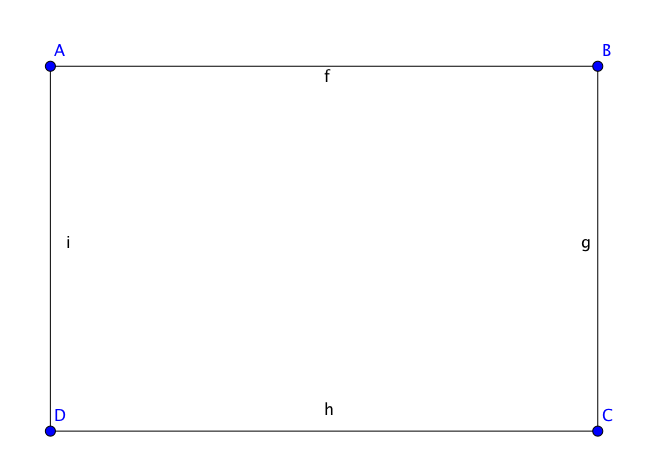
\includegraphics[width=\linewidth]{original_shape}
\caption{Original shape}\label{fig:mouse}
\end{subfigure}\hspace{20 mm}
\begin{subfigure}[b]{.4\linewidth}
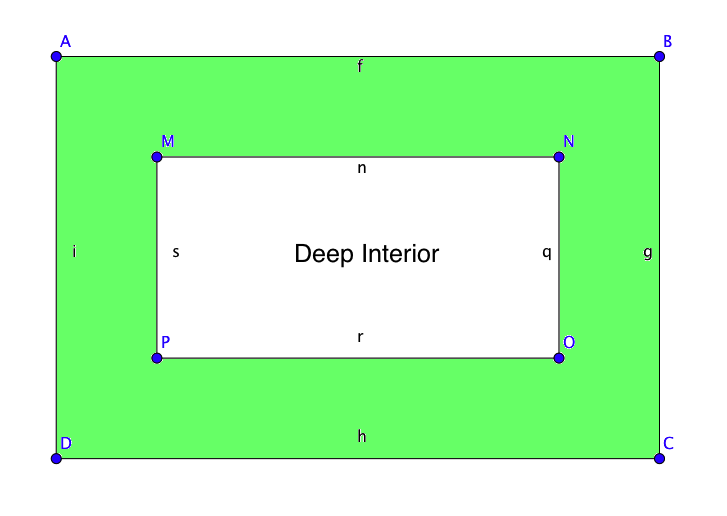
\includegraphics[width=\linewidth]{inner_boundary}
\caption{Inner set $A$ in green}\label{fig:gull}
\end{subfigure}

\begin{subfigure}[b]{.4\linewidth}
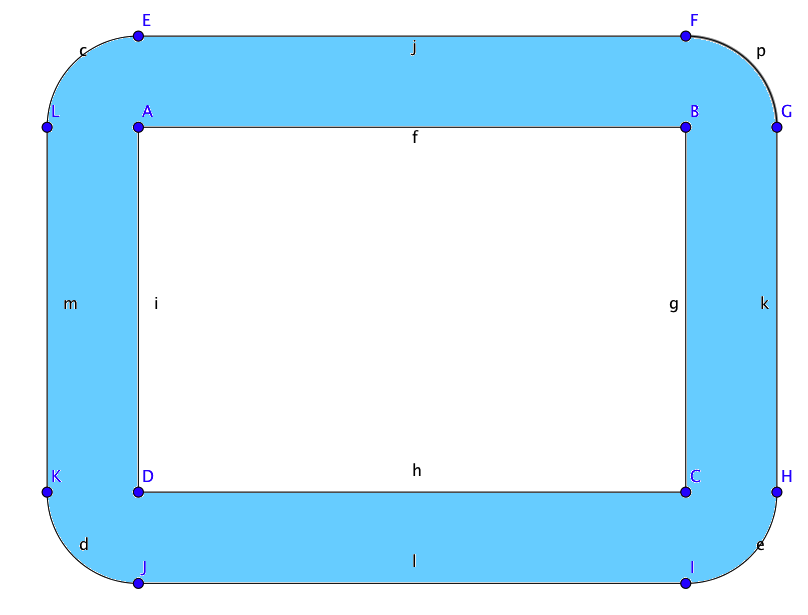
\includegraphics[width=\linewidth]{outer_boundary}
\caption{Outer set $B$ in blue}\label{fig:tiger}
\end{subfigure}\hspace{20 mm}
\caption{Illustration of inner and outer sets for approximate convex hull}
\label{fig:animals}
\end{figure}

\noindent First, we observe that the boundary of the convex hull of $S$ must be contained in the union of $A$ and $B$, that is, it cannot intersect with the deep interior. This is because, for every point $q$ in $O$, there must be some point $s$ in $S$ that is within distance $\epsilon$ of $q$. This means that every point in the deep interior (inside $O$ but not in $A$) will be eventually discarded.
\\

\noindent Now, examine figure 2, which shows the top half of the original rectangle defined by $O$, along with corresponding parts of $A$ and $B$. Regions $C1, C2, E$ are part of the outer set $B$, and $I$ is part of the inner set $A$. In regions $C1$ and $C2$ we will select at most a constant number of points, because it is contained in a circle of radius $\epsilon$. There are OPT such regions. In region $E$, we can use an argument similar to the 1D case to show that we will select, in expectation, at most $O(\log{n})$ points. This is because the height of $E$ is $\epsilon$. The idea is that we can view the line $AB$ as the $x$-axis, and consider the $x$-coordinate of each point in $O$. We will discard every new point in $E$ unless it has $x$-coordinate greater than all the current points we have seen in $E$, or $x$-coordinate lesser than all the current points we have seen in $E$.
\\

\begin{figure}
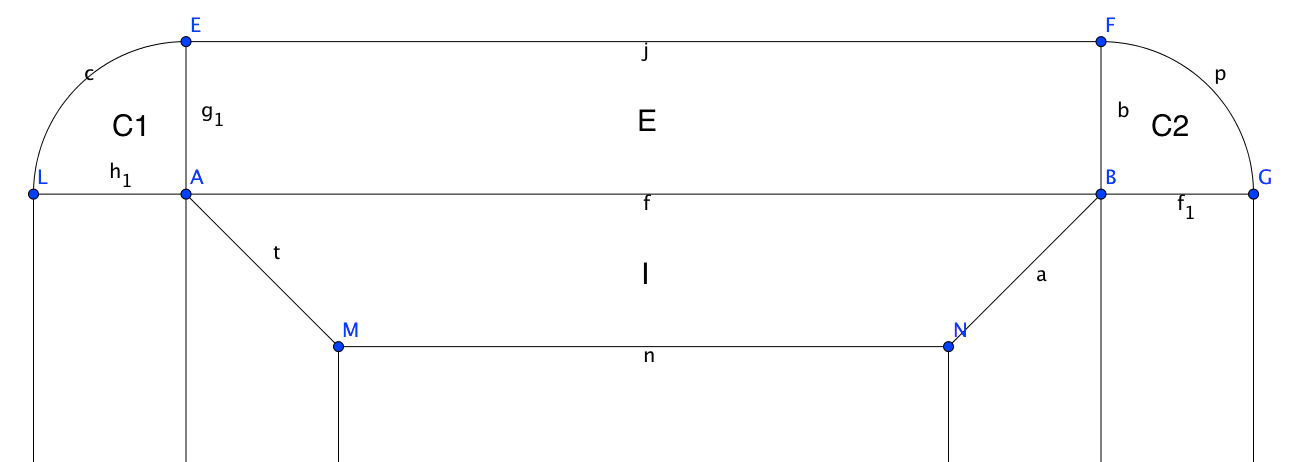
\includegraphics[width=\linewidth]{main_regions}
\caption{Important regions around approximate convex hull}\label{fig:tiger}
\end{figure}

\noindent The same argument applies to $I$. Note that there are OPT such regions, so the total number of points we keep is $O(\mbox{OPT} \cdot \log{n})$. This result is true at every point in the algorithm, so the maximum number of points we keep (at any point in time) is, in expectation, $O(\mbox{MAX-OPT} \cdot \log{n})$. Actually, taking the max is handwavy because the number of points we store is probabilistic, which doesn't interact well with max. So I think we would need to show some kind of high probability bound at each point in the algorithm, and then use union bound. But I'm fairly confident this part will work out.
\\

\noindent This algorithm is unlikely to generalize to higher dimensions. But we could certainly combine it with Harry's and Lin's algorithm when the ambient dimension is higher.

\section{No-Interior Point Clockwise Algorithm}

The setup seems fairly unrealistic and simple. The algorithm is simple but not completely trivial, at each point we need to do some geometric comparisons to figure out what points to throw out. We use storage $O(\mbox{MAX-OPT})$. If there is interest in this algorithm and result, I can write it up. We might use ideas in this algorithm for other algorithms.

\section{Future Directions}

I think we should try to eliminate the $\log{n}$ factor in the random order algorithm. Maybe a modification of something like what we proposed before (keeping a triangle/rectangle/trapezium for each edge of our current approximate convex hull to define the region of space that we have seen points in). I think it might be helpful to first solve the problem for small, fixed, values of MAX-OPT (see goal 4).

\end{document}